\addchap{Press F1 for help}

\minisec{Der Fachschaftsrat}
Nach euren Freunden und Seminargruppenmentoren eure nächste Anlaufstelle.
Wir kümmern uns um eure Probleme oder vermitteln Hilfe.

\minisec{Der Studiendekan}
Neben dem Dekan der Fakultät und seinem Stellvertreter, dem Prodekan, gibt es noch ein weiteres Amt innerhalb der Fakultätsleitung:
den sogenannten Studiendekan.
Er ist für die Angelegenheiten der Lehre in der Fakultät zuständig, bildet den Vermittler zwischen Studenten und Professoren und hilft bei Problemen mit dem Studium allgemein.

Prof. Dr. rer. nat. habil. Weber \\
Büro: APB 1055 \\
Telefon: (0351) 463-38477 \\
E-Mail: gerhard.weber@tu-dresden.de \\

\minisec{Serviceleistung des StuRa}
\begin{itemize}
\item BAföG- und Sozialberatung
\item Rechtsberatung
\item Ausländerberatung
\item Beratung für Studierende mit Kind
\item Beratung zu Anträgen und Förderungsmöglichkeiten
\item Verkauf von Karten für verschiedene Kulturveranstaltungen
\item Material- und Geräteverleih
\end{itemize}

Informationen zu allen Serviceleistungen gibt es im \textit{spiritus rector} und unter \link.
% stura.tu-dresden.de

\minisec{Studienberatung}
Möchtest du dich zu deinem Studiengang beraten lassen oder hast Fragen, dann kannst du dich auch gerne an die Studienberatung wenden.
Studentische Berater sind derzeit Sascha Peukert (Informatik) und Kilian Költzsch (Medieninformatik).
Erreichbar sind sie unter \textit{sascha@ifsr.de} bzw. \textit{koeltzsch@ifsr.de}.
Die Ansprechpartner im Immatrikulationsamt sind auf \link zu finden.
% tu-dresden.de/studium/beratung/studienfachberatung

\minisec{Studium mit Behinderung und chronischer Krankheit}
Unter \link findet ihr Hilfe und Informationen um mit Handicap im Studium gut zurecht zu kommen.
% tu-dresden.de/die_tu_dresden/gremien_und_beauftragte/beauftragte/bfsb

\minisec{Das Prüfungsamt}
Bei Problemen mit der Prüfungseinschreibung, Notenvergabe oder jeglichen Dingen, die mit deinen Prüfungsleistungen zu tun haben ist das Prüfungsamt der entscheidende Ansprechpartner.

Bei Fristüberschreitungen gelten Prüfungen als nicht bestanden und ihr werdet exmatrikuliert.
Unter Umständen seid ihr aber gar nicht schuld am Verstreichen eines Termins.
Dann müsst ihr einen entsprechenden Antrag an den Prüfungsausschuss (PA) stellen.
Gleiches gilt auch, wenn ihr eine frühere Studienleistung (also einen Leistungsnachweis oder das Ergebnis einer Prüfung) anerkannt haben möchtet.
Vorher solltet ihr unbedingt mit euren zwei studentischen Vertretern im Prüfungsausschuss oder mit dem FSR sprechen.
Die Vorsitzenden der Prüfungsausschüsse sind Prof. Baier (Informatik) und Prof. Groh (Medieninformatik), in dringlichen Fällen könnt ihr euch direkt an sie wenden.

Wo: Prüfungsamt, APB 3039/3040 \\
Wann: Di, Do: 12.30 - 15.00 Uhr \\
Mi: 9.00 - 11.00 Uhr \\
Telefon: (0351) 463-38378

Prüfungsamt-Vorsitzende: \\
Prof. Dr. Christel Baier \\
Büro: APB 3006 \\
Telefon: (0351) 463-38548 \\
E-Mail: christel.baier@tu-dresden.de

Prof. Dr. Rainer Groh \\
Büro: APB 2064 \\
Telefon: (0351) 463-39178 \\
E-Mail: rainer.groh@tu-dresden.de

\begin{figure}[h!]
\centering 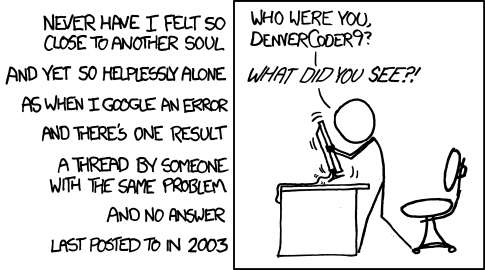
\includegraphics[width=\linewidth]{img/xkcd/wisdom_of_the_ancients.png}
\caption*{{\small \textit{All long help threads should have a sticky globally-editable post at the top saying 'DEAR PEOPLE FROM THE FUTURE: Here's what we've figured out so far ...' (xkcd/979)}}}
\end{figure}
%Bildlink: http://xkcd.com/979
